% !TEX TS-program = xelatex
% !TEX encoding = UTF-8 Unicode
% !Mode:: "TeX:UTF-8"

\documentclass{resume}
\usepackage{graphicx}
\usepackage{tabu}
\usepackage{tabularx}
\usepackage{multirow}
\usepackage{progressbar}
\usepackage{zh_CN-Adobefonts_external} % Simplified Chinese Support using external fonts (./fonts/zh_CN-Adobe/)
\usepackage{tikz}
% \usepackage{NotoSansSC_external}
% \usepackage{NotoSerifCJKsc_external}
% \usepackage{zh_CN-Adobefonts_internal} % Simplified Chinese Support using system fonts
\usepackage{linespacing_fix} % disable extra space before next section
\usepackage{cite}

\newcommand{\hlink}[1]{\href{#1}{#1}}

\begin{document}
\pagenumbering{gobble} % suppress displaying page number

\medskip\noindent
\begin{minipage}{0.7\textwidth}
  \Large{
    \begin{tabu}  { l }
      \scshape{许文郁} \\
      \email{xwymxh@foxmail.com} \\
      \phone{(+86) 18811596155} \\
    \end{tabu}
  }
\end{minipage}
\begin{minipage}{0.3\textwidth}
  \raggedleft
  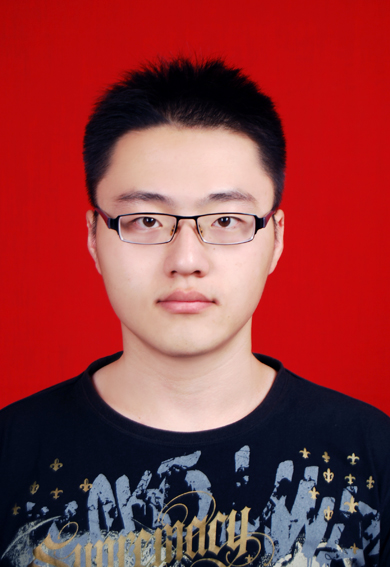
\includegraphics[height=30mm]{me}
\end{minipage}

\section{教育背景}
\datedsubsection{\textbf{北京航空航天大学}}{2017 -- 至今}
\textit{在读硕士研究生}\quad {计算机学院} {2020年1月毕业}
\datedsubsection{\textbf{山西大学}}{2012 -- 2016}
\textit{学士}\quad  {计算机学院}\quad { 软件工程}

\section{技能}
% increase linespacing [parsep=0.5ex]
\begin{itemize}[parsep=0.5ex]
  \item 熟悉Java、JVM、Java并发,熟悉常用的设计模式、数据结构及算法
  \item 熟悉MySQL,了解Redis
  \item 熟悉SSM,了解Zookeeper
\end{itemize}

\section{获奖情况}
\datedline{\textit{全国大学生数学建模竞赛山西赛区二等奖}}{2014 年 8 月}
\datedline{\textit{山西大学优秀毕业生}}{2016 年 7 月}

\section{项目经历}

\datedsubsection{\textbf{基于语义的行人图像生成}}{2018年9月 -- 至今}
\role{VAE,U-net}{研究生课题}
%\begin{onehalfspacing}
\begin{itemize}[topsep = 0 pt, partopsep = 0pt]
  \item 控制生成行人图像的姿态
  \item 相较现有算法,实现了对生成行人的部件级控制
  \item 实验与论文进行中
\end{itemize}
%\end{onehalfspacing}

\datedsubsection{\textbf{某遥感项目}}{2018年5月 -- 2019年1月}
\role{MFC,ZeroMQ}{实验室项目}
%\begin{onehalfspacing}
\begin{itemize}[topsep = 0 pt, partopsep = 0pt]
  \item 利用ZeroMQ传输文本、图像和视频
\end{itemize}
%\end{onehalfspacing}

\datedsubsection{\textbf{电商秒杀系统}}{2017年7月 -- 2017年8月}
\role{SpringBoot,Maven,Mybatis,Redis,RabbitMQ}{个人Demo}
\begin{itemize}[topsep = 0 pt, partopsep = 0pt]
  \item 使用redis做缓存提高访问速度和并发量,减少数据库压力
  \item RabbitMQ 完成异步下单,提升用户体验,削峰和降流
\end{itemize}

\datedsubsection{\textbf{ CTCS-3 列控系统运行状态智能评估系统}}{2013年12月 -- 2014年12月}
\role{SSM,Spark}{大创项目,中国铁道科学研究院}
%\begin{onehalfspacing}
\begin{itemize}[topsep = 0 pt, partopsep = 0pt]
  \item 利用决策树、随机森林算法对降级故障分类
  \item 利用K-means、KNN算法评估列车运行状态
\end{itemize}
%\end{onehalfspacing}

\section{\faInfo\ 其他}
% increase linespacing [parsep=0.5ex]
\begin{itemize}[parsep=0.5ex]
  \item  英语 - 熟练(CET-6)
  \item  性格爱好 - 热情活波;喜欢体育运动(游泳、滑冰等)
\end{itemize}

\end{document}
